\section{Background}
\label{sec-back}
We divide this section into two parts; introducing \smartnics briefly and improving the overall performance by \smartnics are discussed in the first part.  Then, we talk about Artificial Neural Networks (ANN) in the second part.

\subsection{\smartnics Overview}
A glance at Fig. \ref{arhs} reveals two architectures for \smartnics. In the first architecture, \smartnic's processing is located on the path of networking, while in the latter one, Fig. \ref{off-path}, the processing unit is located off the path, communicating with the NIC and the host through PCI Express slot (Peripheral Component Interconnect Express). There are several choices for the \smartnic's processing unit. On-the-shelve CPUs, FPGA, and ASIC are some instances that can be mounted on the \smartnics. In the case of general-purpose CPUs, most of them are ARM-based or MIPS-based wimpy processors.

\par
Owing to the high bandwidth demands of \smartnics, they are connected to hosts over the PCI Express slot, as mentioned in the previous paragraph. However,  PCI Express prompts for extra latency overhead in some cases. Keeping this in mind, either executing an application or offloading part of it into on-path \smartnics can exclude PCI Express extra latency. Nevertheless, FPGAs and CPUs used in on-path \smartnics have limited resources and capabilities. For example, they usually do not support floating-point operations or have a limited memory footprint. It goes without saying that offloaded applications should be modified to be compatible with \smartnics environments and may lose some traits. We will talk about different techniques of modification in the second half of this section, where we discuss ANNs.
\par
Worth to mention, for each kind of \smartnics there are a few brands available in the market; some of them are listed in Table \ref{brands}.

\begin{figure}[ht!]
\centering
    \begin{subfigure}{0.23\textwidth}
        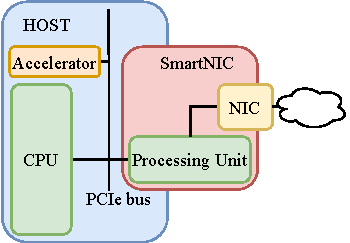
\includegraphics[width=\textwidth]{./figs/on-path.pdf}
        \caption{On-path Architecture}
        \label{on-path}
    \end{subfigure}\hfil
    \begin{subfigure}{0.23\textwidth}
        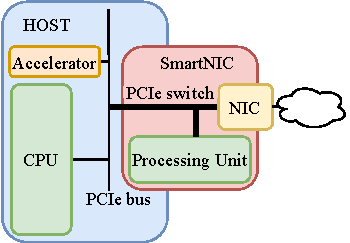
\includegraphics[width=\textwidth]{./figs/off-path.pdf}
        \caption{Off-path Architecture}
        \label{off-path}
    \end{subfigure}\hfil
    \caption{Two architectures for \smartnics}
\label{arhs}
\end{figure}

\begin{table}[hbt!]
\caption{A Few \textit{SmartNICs} Available in the Market}
\label{brands}
\begin{tabular}{|c|c|}
\hline
                   & Available Brands in the Market \\ \hline
On-Path FPGA-based & NetFGPA-SUME \cite{netfpga-sume}                  \\ \hline
On-Path CPU-based  & Liquid IO \cite{liquidio}                     \\ \hline
Off-Path CPU-based & Stingray \cite{stingray} and BlueField \cite{bluefield}        \\ \hline
\end{tabular}
\end{table}

%\subsection{DNNs}
\subsection{Artificial Neural Networks (ANNs)}
\textcolor{red}{[Let's focus our analyses on deep neural networks (DNNs) as these are currently more appealing. Give some background on them. What is a DNN? Where are they used (i.e., most common applications)? What about networking use cases? Give an overview about different architectures (i.e., show they are pretty varied - CNN, RNN, GNN, fully  NN). Talk about different flavors (prunned, compressed, quantized)]}
\textcolor{blue}{Personally, I prefer ANN rather than DNN since some of our implementations are ANN, not necessarily DNN}

In a nutshell, an artificial neural network- or ANN as we call in the rest of the report-is a network of neurons connecting with weighted vertices. An ANN can have one or more than one hidden layer. Also, the nodes/layers can organize different topologies. For instance, Fig. \ref{fcnn} depicts an ANN with two hidden layers, and each node is connected to all the following layer's nodes, knows as Fully Connected ANN. This architecture is use for Multi-layer Perceptron (MLP) classifiers.
\par
\begin{figure}[ht!]
\centering
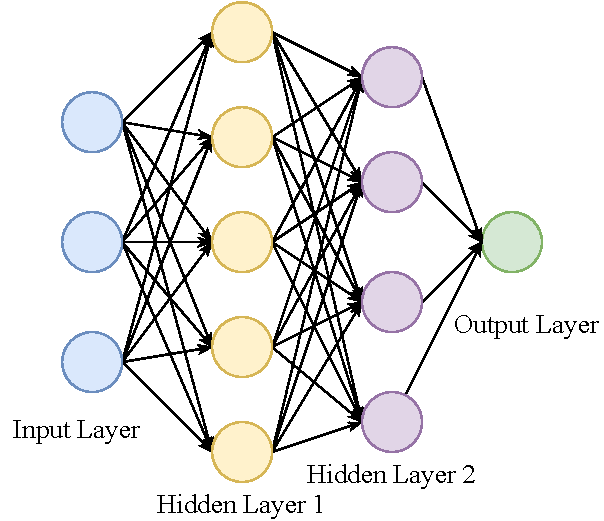
\includegraphics[width=0.4\textwidth]{./figs/fc.pdf}
\caption{An Fully Connected ANN with 2 hidden layers}
\label{fcnn}
\end{figure}
\par
Furthermore, an ANN will be called a Deep Neural Network (DNN) if it has many layers. In more detail, various architectures are introduced for DNN solving different complex problems. Some notable examples are Convolutional Neural Networks (CNNs) and Recurrent Neural Networks (RNNs). The former one is vastly used for video analysis and image classification. Yet, Natural Language Processing is one of use cases for the latter one. 
\par
As has been mentioned before, \smartnics have limited resources. On the other hand, ANNs are resource-hungry applications. Consequently, the original ANNs applications cannot execute on the \smartnics without any modifications. Here, three solutions are listed for reducing the size of any ANNs, including fully connected NNs and DNNs.
\begin{itemize}
  \item \textbf{Compressing}: In this method, the original model is converted to a compressed one via the framework's tools. The compressed one has 2x-4x less size without a prominent loss in the outputs (less than 0.5\% in our results). An example of this method is TensorFlow lite \cite{tflite}.
  \item  \textbf{Quantization}: In this method, more miniature data types are replaced with original data types. In other words, the quantized network has the same topology while the weights of vertices change. In the AI area, using 64bits or 32bits floating-point numbers is very common.  Hence, replacing them with 8bit width data types drops the size significantly. Some studies go further and use only one bit for quantization, generating Binarized Neural Networks (BNNs). It goes without saying that the quantized model is not as accurate as of the original model.
  \item  \textbf{Pruning}: The idea behind this method is to remove the vertices with small weights, or the vertices do not affect the output that much. Therefore, the topology becomes simpler here.
\end{itemize}

Up to here, we have provided adequate background regarding ANNs. The question coming to mind is \textbf{which ANN do we study in our project?}
As we have mentioned, each ANN is suitable for a specific problem. The same in the Computer Networks area; based on the nature of the issue, the ANN's architecture would be chosen. For packet classification, fully connected ANNs provide acceptable accuracy. However, for analysis MPLS configuration, a deep NN provides a viable outcome \cite{8999396}. Here, we will evaluate two kinds. The first one would be VGG16 \cite{simonyan2014very}, which is basically a deep NN for Image Classification. The second one would be a fully connected ANN for anomaly detection. We try to avoid quantizing or pruning the models, and utilizing the original model or the compressed one to keep the models accurate in our project.